\documentclass[../RASD.tex]{subfiles}

\usepackage{geometry}

\begin{document}
    \graphicspath{{\subfix{assets/section_2/}}}

    In this section a description of some \textit{typical scenarios}, the \textit{Product functions} (see \ref{subsec:product_functions}) offered by the CKB platform and the \textit{UML class diagram} (see \ref{subsubsec:class_diagram}) are presented.
    Later on in section also assumption, dependencies and constrains are discussed (see \ref{subsec:user_characteristics}, \ref{subsec:assumption_dependencies_and_constrain}).
    \subsection{Product perspective}\label{subsec:product_perspective}
    \subsubsection{Scenarios}\label{subsubsec:scenarios}
        \begin{enumerate}
            \item {Mister Russo has just started a new career in software development and wants to become better at coding.
            For this reason he wants to create an account on the platform.
            \begin{itemize}
                \item {He opens up the application and clicks on the "Sign Up" button;}
                \item {He inserts all the mandatory information in the provided fields and presses the "Confirm" button;}
                \item {The system checks that e-mail has not been used before.
                After passing the verification a confirmation notification is sent to mister Russo;}
                \item {He checks his notification to see if he has received the confirmation of successful creation of the account.}
            \end{itemize}}
            \item {Mister Ferrari is a well known business owner that wants to organize an awarded competition between his employees.
            To fulfill his goal mister Ferrari decides to create a tournament.
            Moreover, since mister Ferrari does not know anything about software development, he decides to invite some coworker with the intent to manage the tournament. 
            \begin{itemize}
                \item {He opens up the application and logs-in;}
                \item {He navigates to the tournament section;}
                \item {He clicks on "Create a new Tournament" button;}
                \item {He inserts the tournament's name and deadline in the provided fields and presses the "Continue" button;}
                \item {The system checks that no other tournament has the same name.
                Upon a successful verification a confirmation notification is sent to mister Ferrari;}
                \item {The system generates a notification informing all the users of CKB platform that a new tournament has been created;}
                \item {He check his notifications to see if he has received the confirmation of the successful creation of the tournament.
                At this point he can invite his collaborators;}
                \item {He clicks on "Tournament" page and then selects his own tournament;}
                \item {He clicks on "Manage educators" button;}
                \item {He clicks on the "+" button and search the collaborators he wants to invite using their e-mail or nickname;}
                \item {He clicks on "Invite educators" button.}
            \end{itemize}}
            \item {Miss Esposito is one of the most skilled programmers in the company where she works.
            Because of this her boss asked her to create challenges for the company's tournament.
            The boss has already invited miss Esposito as a tournament's collaborator.
            \begin{itemize}
                \item {She checks her notifications to see if she has received the invite;}
                \item {She clicks on the link on the notification to accept the invite to the tournament.
                The link redirects her to the platform login page;}
                \item {She logs-in, navigates to the "Tournament" section and selects the tournament where she has been invited as an educator;}
                \item {She clicks on "New Battle" button;}
                \item {She clicks on "Upload" button in order to upload the code kata;}
                \item {She fills up, using the provided fields, all the required information including:
                \begin{enumerate}
                    \item {minimum number of students per group}
                    \item {maximum  number of students per group}
                    \item {registration deadline}
                    \item {final submission deadline}
                    \item {additional configuration for scoring}
                \end{enumerate}}
                \item {She clicks on "Create new battle" button;}
                \item {The system generates a notification informing all users subscribed to the battle's tournament that a new battle is available.}
            \end{itemize}}
            \item {Miss Bianchi is subscribed to the platform.
            Since she has some free time she wants to subscribe to the tournament she was notified.
            She has already checked her notification containing all the information about the tournament.
            \begin{itemize}
                \item {She opens up the application and logs-in;}
                \item {She navigates to the tournament section;}
                \item {She clicks on the corresponding tournament name that she has read about on her notification;}
                \item {She clicks on "Subscribe" button.}
            \end{itemize}}
            \item {Miss Romano and mister Colombo are close friends that would like to team up and compete in a battle.
            To do so they decide to create a group.
            Both of them are already subscribed to the same battle, and they establish a priori that Miss Romano will create the group on the platform.
            \begin{itemize}
                \item {Miss Romano opens up the application and logs-in;}
                \item {She navigates to the tournament section;}
                \item {She clicks on the corresponding tournament name in which both of them are already subscribed;}
                \item {She clicks on the corresponding battle name in which both of them are already subscribed;}
                \item {She clicks on "Create a group" button;}
                \item {She inserts the name of the group;}
                \item {The system checks that no other group with the same name is present in the context of the same battle;}
                \item {She clicks on "Confirm creation" button;}
                \item {She clicks on "Manage group" button;}
                \item {She clicks on "Invite new user" button;}
                \item {She searches the collaborators she wants to invite using their e-mail or nickname;}
                \item {She clicks "Invite" button.}
                \item {Mister Colombo awaits for the notification that contains the invite from Miss Romano;}
                \item {He opens up the notification;}
                \item {The system redirects him to the application;}
                \item {He logs-in and accept the invite;}
            \end{itemize}}
            \item {The group of students named "PythonMasters" wants to deliver the solution of "C Recursion" battle in which they are competing.
            PythonMasters has already forked the repository in order to access the code kata.
            \begin{itemize}
                \item {They set up an automated workflow, using the repository service that informs CKB platform when a push action occurs;}
                \item {They push their solution onto the repository;}
                \item {They open up the application and log-in;}
                \item {They navigate to the tournament section and select the tournament in which they are competing;}
                \item {They select "C Recursion" battle;}
                \item {They await for the system to complete automated code evaluation;}
                \item {They can now visualize their score.}
            \end{itemize}}
            \item {Miss Bruno, educator of the tournament, wants to personally review the score of a battle.
            The battle has previously been created such that it needs manual code evaluation.
            \begin{itemize}
                \item {She opens up the application and logs-in;}
                \item {She navigates to the tournament section and selects the tournament in which the battle is being hosted;}
                \item {She clicks on "Review submissions" button;}
                \item {She reviews the solutions.}
            \end{itemize}}
            \item {Mister Ricci has created a battle with the wrong code kata and so he decides to remove such battle.
            He is already logged into the platform.
            \begin{itemize}
                \item {He navigates to the tournament section and selects the tournament in which he has previously created the battle;}
                \item {He navigates to the current battle;}
                \item {He clicks on "Delete battle" button;}
                \item {He clicks on "Yes, I'm sure" button;}
            \end{itemize}}
            \item {Miss Marino, given the new schedule, needs to close a tournament before the deadline expires.
            She is the TO of the aforementioned tournament and she is already logged into the platform.
            \begin{itemize}
                \item {She navigates to the tournament section and selects the tournament she wants to close;}
                \item {She clicks on "Close tournament" button;}
                \item {She clicks on "Yes, I'm sure" button;}
            \end{itemize}}
        \end{enumerate}
    \newpage
    \newgeometry{left=1.5cm, right=1.5cm, top=2em}
    \subsubsection{Class diagram}\label{subsubsec:class_diagram}
    In the UML diagram all the main entities of the system are shown. 
    CKB platform is principally composed by two principal entities: \textit{User} and \textit{Tournament}. 
    The \textit{User} entity represents all the users of the platform and models the interaction of the user with the system by a dynamic specialization into \textit{Student} and \textit{Educator} entities.
    This ensures flexibility for the end user of the platform that can be at the same time a student and an educator.
    Hence, the user can compete in a tournament and at the same time create its own tournament, all without the need of creating multiple accounts.\\
    The \textit{Tournament} entity represents the tournaments created by the educators.
    This class models the competitions between students and the interaction of the educators with the system.
    From here a \textit{Student} can enroll in a \textit{Battle}, created by an \textit{Educator}, and form \textit{Group} with other students.
    \begin{figure}[h!]
        \centering
        \hspace*{-2cm}
        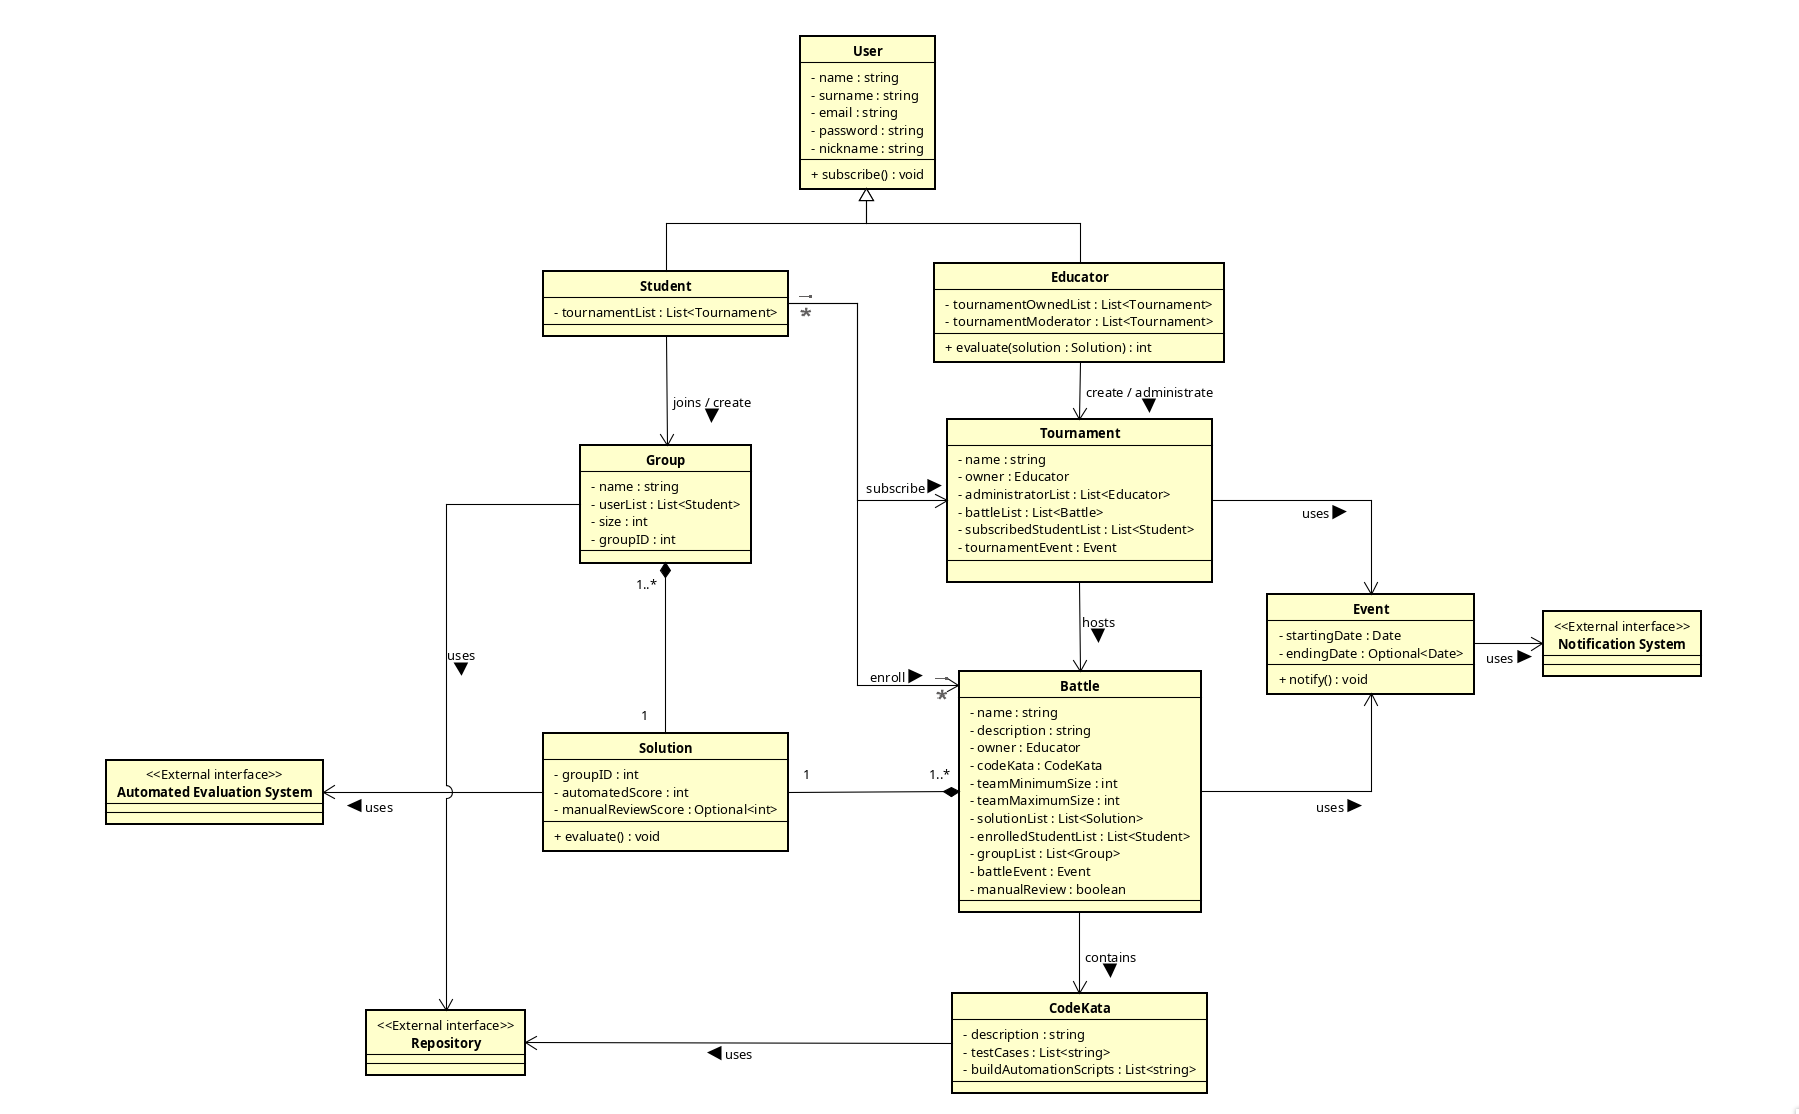
\includegraphics[width=1.2\textwidth]{../assets/section_2/class_diagram.png}
        \hspace*{2cm}
    \end{figure}
    \newpage
    \restoregeometry

    \newgeometry{left=1.5cm, right=1.5cm}
    \subsection{Product functions}\label{subsec:product_functions}
    \begin{itemize}
        \item {\textbf{Sign-up}: let users sign-up through their e-mail and password.
        \begin{figure}[h]
            \centering
            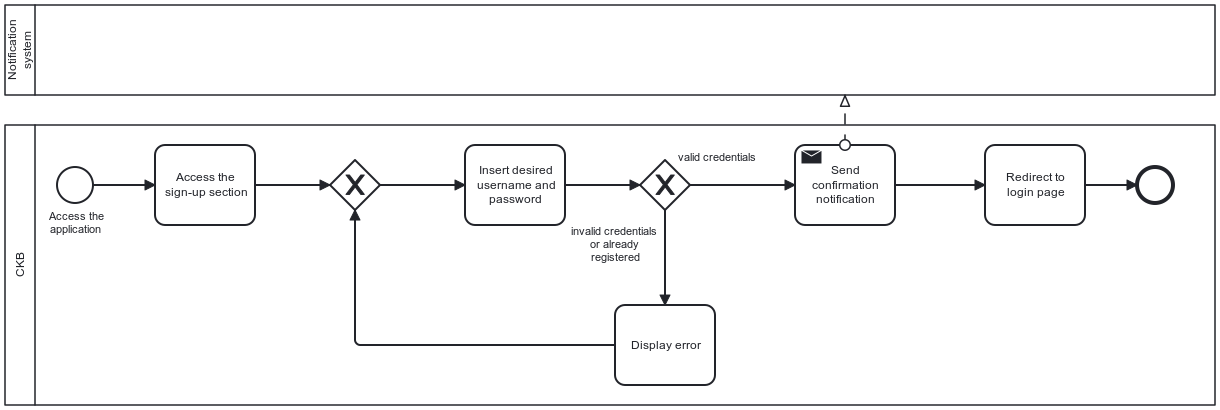
\includegraphics[width=\textwidth]{../assets/section_2/sign_up_definitive.png}
            \caption{Sign-up to CKB platform.}
            \label{img:bpmn_login}
        \end{figure}
        \newpage
        }
        \item {\textbf{Create a tournament}: let educators create a tournament.
        \begin{figure}[h]
            \centering
            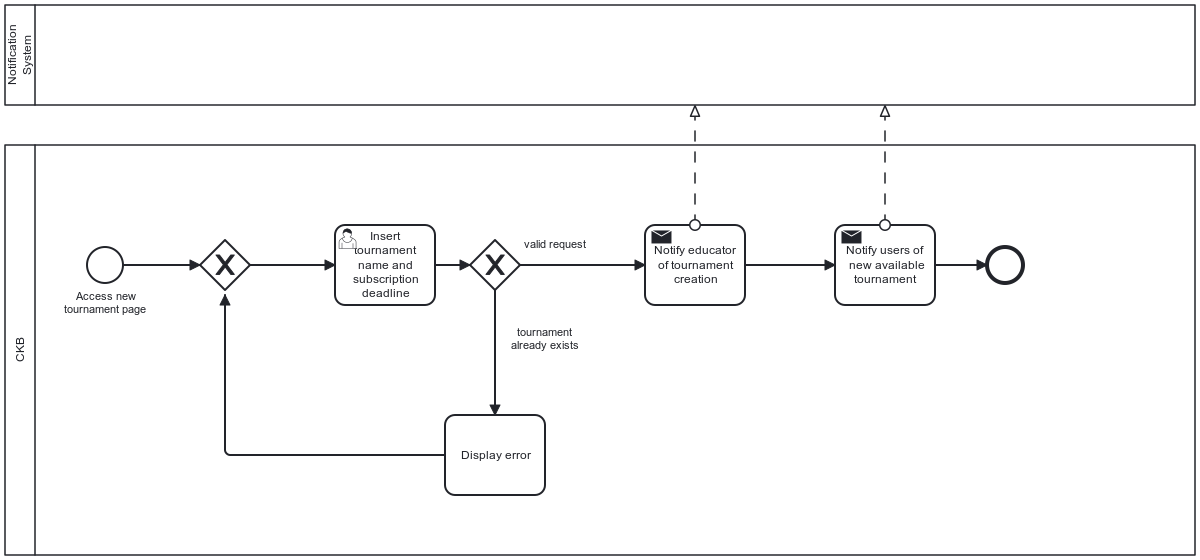
\includegraphics[width=\textwidth]{../assets/section_2/create_tournament_definitive.png}
            \caption{Create a tournament.}
            \label{img:bpmn_create_tournament}
        \end{figure}
        \newpage
        }
        \item {\textbf{Invite educator}: let the \textit{TO} invite other educators.
        \begin{figure}[h]
            \centering
            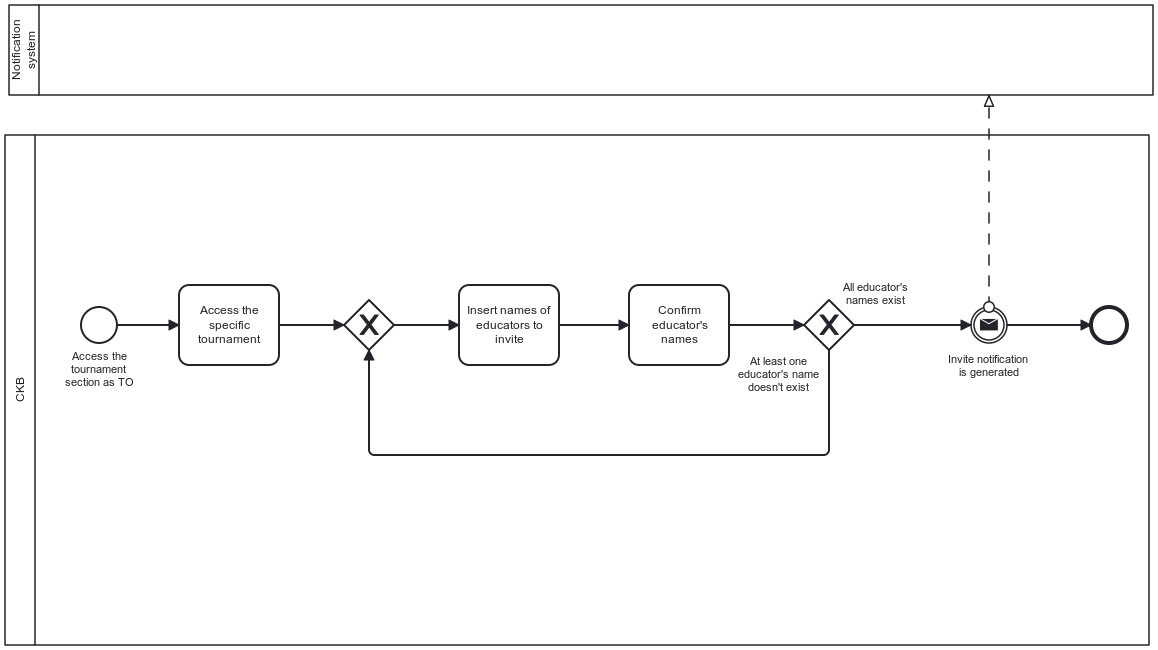
\includegraphics[width=\textwidth]{../assets/section_2/InviteEducator_definitive.png}
            \caption{Manage a tournament as \textit{TO}.}
            \label{img:bpmn_manage_tournament}
        \end{figure}
        \newpage
        }
        \item {\textbf{Create a battle}: let educators create a battle.
        \begin{figure}[h]
            \centering
            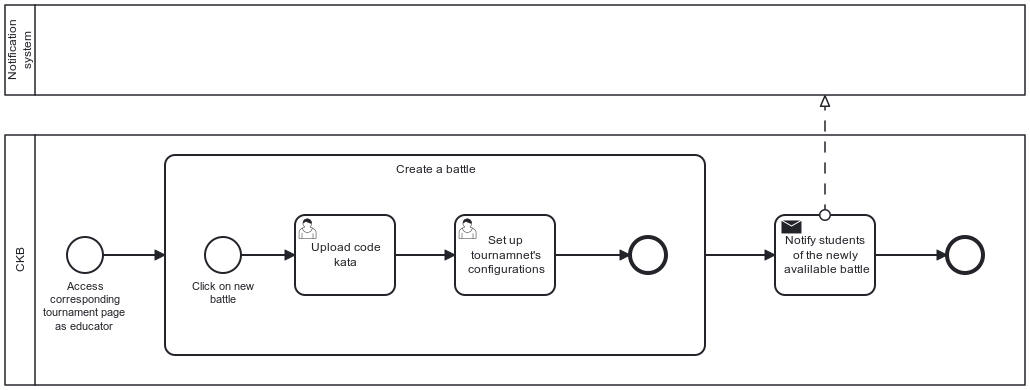
\includegraphics[width=\textwidth]{../assets/section_2/create_battle_definitive.png}
            \caption{Create a battle.}
            \label{img:bpmn_create_battle}
        \end{figure}
        \newpage
        }
        \item {\textbf{Group creation}: let students enrolled into the same battle to create a group.
        \begin{figure}[h]
            \centering
            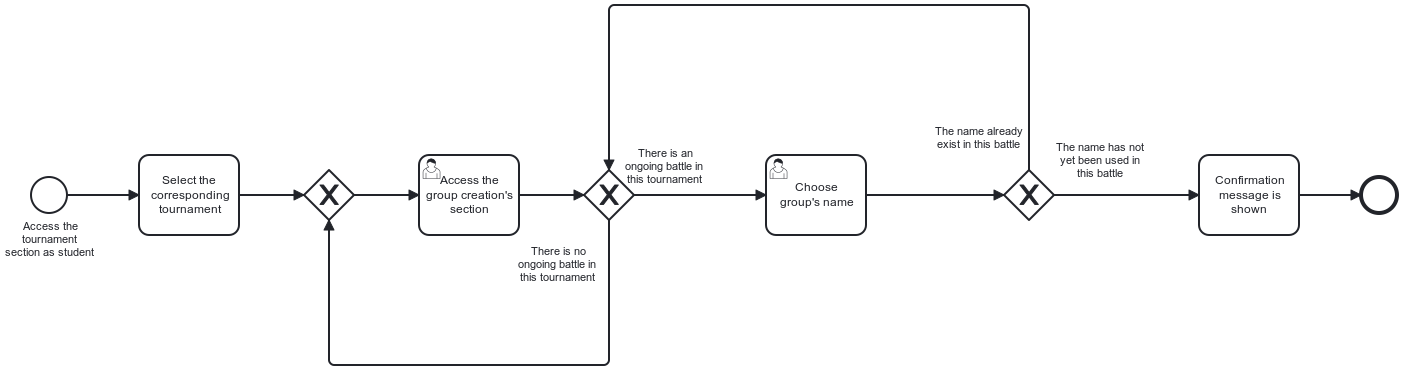
\includegraphics[width=\textwidth]{../assets/section_2/group_creation_definitive.png}
            \caption{Let students enrolled intto the same battle to create a group.}
            \label{img:bpmn_group_creation}
        \end{figure}
        \newpage
        }
        \item {\textbf{Enroll in a battle}: let a student join a battle in a tournament.
        \begin{figure}[h]
            \centering
            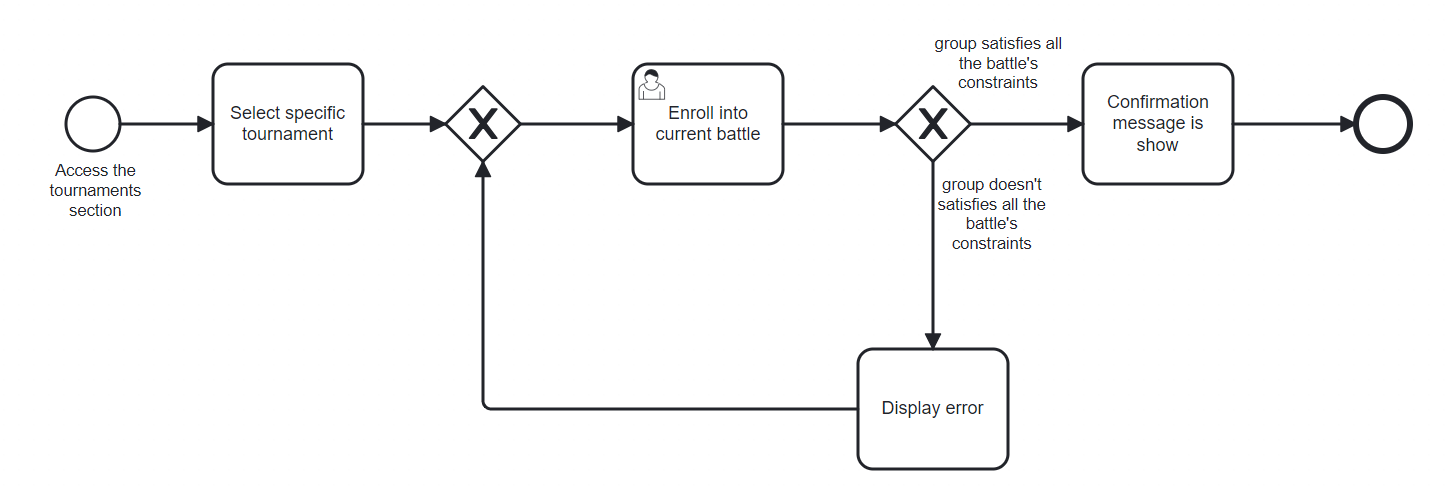
\includegraphics[width=\textwidth]{../assets/section_2/enroll_in_a_battle_definitive.png}
            \caption{Join a battle in a tournament.}
            \label{img:bpmn_enroll_in_a_battle}
        \end{figure}
        \newpage
        }
        \restoregeometry
        \item {\textbf{Group delivers a solution}: let groups of students upload their solution\\
        within the context of a battle and view their personal score.
        \begin{figure}[h!]
            \centering
            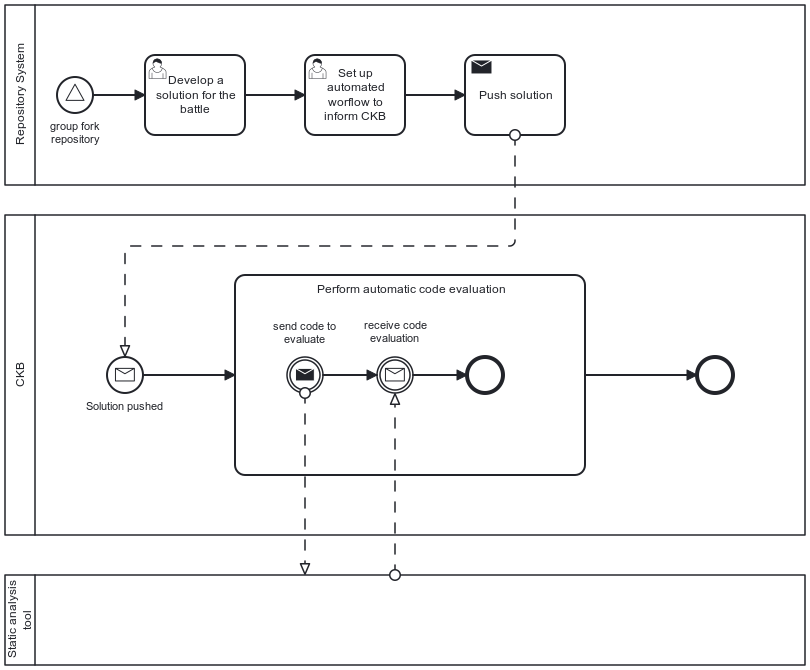
\includegraphics[width=\textwidth]{../assets/section_2/group_upload_solution_definitive.png}
            \caption{Let gropus upload their solution and see their result.}
            \label{img:bpmn_group_upload_solution_and_see_results}
        \end{figure}
        \newpage
        }
        \newgeometry{left=1.5cm, right=1.5cm}
        \item {\textbf{Educator manual review}: let the tournament's educators give a score to a group's solution within the context of a battle.
        \begin{figure}[h!]
            \centering
            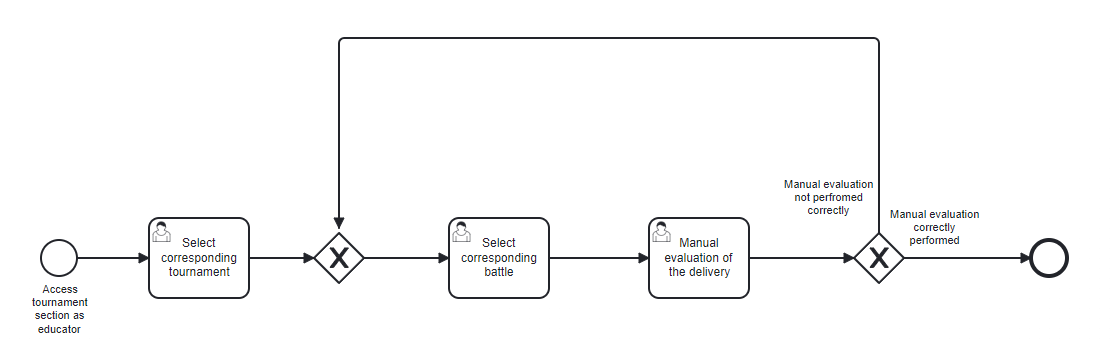
\includegraphics[width=\textwidth]{../assets/section_2/educator_code_review_definitive.png}
            \caption{Let tournament's educators give an additional evaluation to a group's score.}
            \label{img:bpmn_educator_code_review}
        \end{figure}
        \newpage
        }
    \end{itemize}
    \newpage
    \restoregeometry
    \subsection{User characteristics}\label{subsec:user_characteristics}
    The application has been designed for:
    \begin{itemize}
        \item anyone who wants to become better at coding;
        \item any organization or physical person who wants to create online, software development related, competitions.
    \end{itemize}
    For this reasons, the potential user base includes all the people that have a connection, whether personal or business related\footnote{This aside is intended to emphatize the fact that the platform can be used by users that have personal interest in software development, such as an hobby, but also by users that have professional careers in the field.}, with the world of software development.
    Users should be capable of interacting with the application and be in posses of a valid mailbox.
    \newpage
    \subsection{Assumption, dependencies and constrains}\label{subsec:assumption_dependencies_and_constrain}
    \begin{itemize}
        \item {\textbf{D1}: Users have internet access while using the application}
        \item {\textbf{D2}: Users have only one account\footnote{To avoid multiple accounts per user}}
        \item {\textbf{D3}: Users device always send correct data to the application regarding its specifications\footnote{For example the device type(smartphone, laptop, ...) or the screen width}}
        \item {\textbf{D4}: The repository service is reliable and works 99.9\% of the time}
        \item {\textbf{D5}: Users have the ability to interact and correctly use the repository platform}
        \item {\textbf{D6}: Users notification system is reliable and works 99.9\% of the time}
        \item {\textbf{D7}: Users won't block notifications coming from the application}
        \item {\textbf{D8}: The automated evaluation system is reliable and works 99.9\% of the time}
        \item {\textbf{D9}: Users who are members of the same group will contribute equally to the delivery}
        \item {\textbf{D10}: Users won't receive any external help from a person not in their group while competing in a battle}
        \item {\textbf{D11}: Educator's manual review of the delivery is unbiased}
    \end{itemize}\newpage
    
\end{document}
